\documentclass{article}
\usepackage{graphicx}
\usepackage{amsmath}
\usepackage{amsthm}
\usepackage{wrapfig}
\usepackage{algorithm}
\usepackage{booktabs}
\usepackage{subcaption}
\usepackage{tikz}
\usepackage{algorithmic}
\usetikzlibrary{spy}
\usepackage{listings}
\newtheorem{theorem}{Theorem}
% Examples of custom/rare figures with mixed content

\begin{document}

% see issue ar5iv#83
\begin{table*}[t]
  \footnotesize
  \resizebox{0.36\columnwidth}{!}{
  \begin{minipage}[t]{0.4\textwidth}
    \begin{tabular}{cc}
      \toprule
      Head & Meta \\
      \midrule
      Body & Content \\
      \bottomrule
    \end{tabular}
  \end{minipage}}
  \hspace{15em}
  \resizebox{0.36\columnwidth}{!}{
  \begin{minipage}[t]{0.4\textwidth}
    \begin{tabular}{cc}
    \toprule
    Head 2 & Meta 2 \\
    \midrule
    Body 2 & Content 2 \\
    \bottomrule
    \end{tabular}
  \end{minipage}}
  \caption{table with two resized, minipage, tabulars}
\end{table*}
\clearpage

% \includegraphics as a node in tikz, see ar5iv#215
\begin{figure*}
  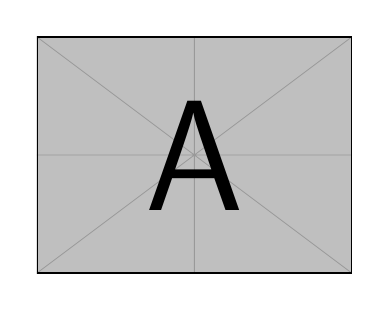
\begin{tikzpicture}
    \begin{scope}[spy using outlines={rectangle,blue,magnification=2.5,size=3cm}]
    \node {	\includegraphics[height=3cm]{example-image-a}};
    \end{scope}
  \end{tikzpicture}

  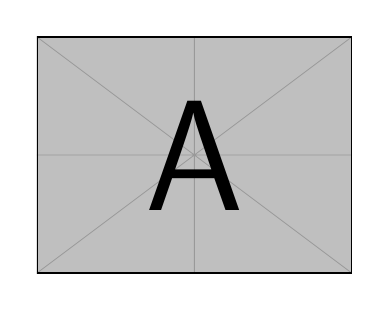
\begin{tikzpicture}
    \begin{scope}[spy using outlines={rectangle,blue,magnification=2.5,size=3cm}]
    \node {	\includegraphics[height=3cm]{example-image-a}};
    \end{scope}
  \end{tikzpicture}
  \caption{tikz nodes with includegraphics}
\end{figure*}
\clearpage

% math array with subfloat
\begin{figure}
  $ \begin{array}{cc}
    \subfloat[]{\includegraphics[width=3cm]{example-image-a} \label{array:subfig1}} &
    \subfloat[]{\includegraphics[width=3cm]{example-image-a} \label{array:subfig2}}
  \end{array} $
  \caption{math array figure}
  \label{array:fig}
\end{figure}
Testing \ref{array:subfig1} and \ref{array:subfig2} inside \ref{array:fig}.
\clearpage

\begin{wrapfigure}{r}{0.35\textwidth}
  \vspace{-2.25em}
  \centering
  \begin{minipage}{\linewidth}
  \begin{algorithm}[H]
  \caption{A Wrapped Algorithm}
  1- mock algorithm with just enough textual content.\\
  2- mock algorithm with just enough textual content.\\
  3- mock algorithm with just enough textual content.
  \end{algorithm}
  \end{minipage}
  \vspace{-1em}
\end{wrapfigure}
\vspace{-2mm}
\paragraph{Lorem ipsum dolores} Lorem ipsum dolor sit amet, consectetur adipiscing elit, sed do eiusmod tempor incididunt ut labore et dolore magna aliqua. Nibh sit amet commodo nulla. Id nibh tortor id aliquet lectus proin nibh. Quam quisque id diam vel quam elementum. Ut porttitor leo a diam sollicitudin tempor id. Pulvinar etiam non quam lacus suspendisse faucibus interdum posuere lorem. Magnis dis parturient montes nascetur ridiculus mus mauris. Quam nulla porttitor massa id. Mattis ullamcorper velit sed ullamcorper morbi tincidunt ornare massa eget. Fringilla urna porttitor rhoncus dolor. Eget mauris pharetra et ultrices neque ornare aenean. Lorem sed risus ultricies tristique nulla. Nunc lobortis mattis aliquam faucibus purus in massa. Purus ut faucibus pulvinar elementum integer enim neque. Cras sed felis eget velit aliquet sagittis. Odio aenean sed adipiscing diam donec adipiscing. Lacus sed turpis tincidunt id aliquet. Blandit volutpat maecenas volutpat blandit. Donec massa sapien faucibus et molestie. Blandit aliquam etiam erat velit.
\clearpage

% Explicit tabular arrangement with resizebox
\begin{figure*}[htbp]
	\centering
  \begin{tabular}{ccc}
 		\resizebox{5.0cm}{!}{\includegraphics{example-image-a}}&
		\resizebox{5.0cm}{!}{\includegraphics{example-image-a}}&
		\resizebox{5.0cm}{!}{\includegraphics{example-image-a}}\\
		\resizebox{5.0cm}{!}{\includegraphics{example-image-a}}&
		\resizebox{5.0cm}{!}{\includegraphics{example-image-a}}&
		\resizebox{5.0cm}{!}{\includegraphics{example-image-a}}
   \end{tabular}
	\caption{a tabular + resizebox}
\end{figure*}
\clearpage


% two subfigures and an itemize
\begin{figure}
  \begin{minipage}[t]{0.4\textwidth}
    \includegraphics[width={0.4\textwidth}]{example-image-a}
  \end{minipage}
  \begin{minipage}[t]{0.4\textwidth}
    \includegraphics[width={0.4\textwidth}]{example-image-a}
  \end{minipage} \\
  \begin{center}\begin{itemize}
    \item post-minipage item 1
    \item post-minipage item 2
    \item post-minipage item 3
  \end{itemize}\end{center}
  \caption{Two minipages and an itemize}
\end{figure}
\clearpage

% listing, itemize, enumerate, inline math, display math, para text
% footnotes, equation group, quote, theorem?
\begin{figure}
  \begin{lstlisting}
    listing
  \end{lstlisting}%
  \begin{itemize}\item itemize 1 \end{itemize}\footnote{note1}.%
  \begin{enumerate}\item enumerate 1 \end{enumerate}%
  $ \sqrt{x} = 0 $%
  \[ E = mc^2 \]%

  Some paragraph text

  \begin{eqnarray*}
    A&=&B,\\
    C&=&D,\\
  \end{eqnarray*}
  \begin{quote}Quote me later\end{quote}%
  \begin{theorem} mock theorem \end{theorem}%
  \begin{verbatim} some verbatim $#! stuff \end{verbatim}%
  \caption{Highly mixed figure}
\end{figure}
\clearpage

% manual horizontal panels with a Trailing note and punct
\begin{figure}
  \includegraphics[width=0.33\textwidth]{example-image-a}\hspace{2cm}%
  \includegraphics[width=0.33\textwidth]{example-image-a}%
  \footnote{Note}.
  \caption{Caption}
\end{figure}
\clearpage

% 3 algorithms in minipages, taken from arXiv and anonymized
\begin{figure*}[tb]
  \begin{minipage}{0.56\textwidth}

  \vspace{-10px}
  \begin{algorithm}[H]
    \caption{Algorithms in minipage}
    \label{alg:main}
  \begin{algorithmic}[1]
    \REQUIRE line
    \STATE line
    \STATE line
    \STATE line
    \STATE line

    \FOR{$\text{line}$}

      \STATE line
      \STATE line
    \ENDFOR
    \STATE
    \STATE line
    \WHILE{line}
      \STATE line
      \WHILE{line}
        \STATE line
        \STATE \textbf{line}
        \STATE \hspace{16px} line
        \STATE \hspace{16px} line
        \STATE \hspace{16px} line
        \STATE \hspace{16px} line

        \STATE \textbf{line} line:
        \STATE \hspace{16px} line
        \STATE \hspace{16px} line
        \STATE \hspace{16px} line
        \STATE \hspace{16px} line
        \STATE \hspace{16px} \hspace{16px} line
        \STATE \hspace{16px} \hspace{16px} line
        \STATE \hspace{16px} line
        \STATE \hspace{16px} line

      \ENDWHILE
      \STATE
      \STATE line
      \STATE line \COMMENT{line}
      \STATE line
      \STATE line
    \ENDWHILE
    \STATE
    \FOR{$\text{line}$}
      \STATE line
    \ENDFOR

    \STATE \textbf{return} line

  \end{algorithmic}
  \end{algorithm}
  \vspace{-18px}
  \end{minipage}\hspace{8px}
  \begin{minipage}{0.42\textwidth}

  \vspace{-10px}
  \begin{algorithm}[H]
    \caption{{\color{blue}line}}
    \label{alg:rpc}
  \begin{algorithmic}[1]
    \REQUIRE line
    \STATE line
    \FOR{$\text{line}$}
      \STATE line
    \ENDFOR

    \WHILE{line}
      \STATE line
      \FOR{$\text{line}$}
        \STATE line
        \STATE line
        \STATE \hspace{16px} line
        \STATE line
      \ENDFOR
      \STATE line
    \ENDWHILE

  \end{algorithmic}
  \end{algorithm}
  \vspace{-18px}
  \begin{algorithm}[H]
    \caption{{\color{blue}line}}
    \label{alg:replace}
  \begin{algorithmic}[1]
    \REQUIRE line
    \STATE line
    \STATE line
    \STATE line
    \STATE \hspace{8px} line
    \STATE line
    \STATE line
    \WHILE{line}
      \STATE \hspace{-4px} line
      \STATE \hspace{-4px} line
      \STATE \hspace{4px} line
      \STATE \hspace{4px} line
      \STATE \hspace{4px} line
      \STATE \hspace{4px} line
      \STATE \hspace{4px} line
      \STATE \hspace{4px} line
      \STATE \hspace{-4px} line
      \STATE \hspace{4px} line
      \STATE \hspace{4px} line
      \STATE \hspace{12px} line
      \STATE \hspace{4px} line
    \ENDWHILE
    \STATE \textbf{return} chain
  \end{algorithmic}
  \end{algorithm}
  \vspace{-18px}\end{minipage}
  \vspace{-5pt}
\end{figure*}

\end{document}